\chapter{Supplementary: thermal forward modelling operator}
\label{c:ThermModel}

The thermal parameter fitting strategy and the obtained thermal model (chapter~\ref{c:ThermAppl}) rely on a finite-difference solver for the steady-state heat equation.
Its fundamental relationship can expressed in the following vector form:
\begin{equation}
    \label{suppl:eq:heateq}
    \bm{\nabla} \cdot ( k(\bm{x}) \bm{\nabla} T(\bm{x}) ) = - A(\bm{x})
\end{equation}
with $k$ thermal conductivity (considered isotropic), $T$ temperature, $A$ heat production per unit of volume, and $\bm{x}$ position vector.
This form results from simplification of the well known heat equation in its full form \parencites{Fourier1822,Carslaw1959}, a heat source term included:
\begin{equation}
    \label{suppl:eq:fullheateq}
    \frac{\partial T}{\partial t} = \alpha \bm{\nabla}^2 T + \frac{A}{\rho c_p}
\end{equation}
where $t$ denotes time and $\alpha$ `thermal diffusivity', i.e. the product of thermal conductivity ($k$), density ($\rho$), and specific heat ($c_p$).
The steady-state assumption imposes:
\begin{equation}
    \label{suppl:eq:steadystate}
    \frac{\partial T}{\partial t} = 0
\end{equation}
This allows simplification of Eq.~\ref{suppl:eq:fullheateq} to:
\begin{equation}
    \label{suppl:eq:steadystatefullheateq}
    0 = \rho c_p \left( k \bm{\nabla}^2 T + A \right)
\end{equation}
therefore:
\begin{equation}
    \label{suppl:eq:steadystatefullheateq_simplified}
    k \bm{\nabla}^2 T = - A
\end{equation}
which is equivalent to Eq.~\ref{suppl:eq:heateq}, as expressed above \parencite[e.g. ][, chapter 3]{stuwe2007geodynamics}.
This is a partial differential equation (PDE), in the form of Poisson's equation ($\bm{\nabla}^2 \phi = f$, for two generic $\phi$ and $f$ functions).

Analytical solution exist: plenty are available for specific cases of geological interest \parencites(see e.g. )()[][chapter 4.6]{Turcotte2014_geodynamics}[][chapter 3.4]{stuwe2007geodynamics}.
As pointed out by \textcite{Gerya2010} a pitfall of analytical methods for PDE solution is that they are "restricted to relatively simple problems" \parencite[][chapter 3.1]{Gerya2010}.
To analytically express the distribution of parameters' fields (e.g. $A$, $k$) is often cumbersome, sometimes impossible.
For the purposes of this thesis, a solver to the steady-state heat equation based on the finite-difference method \parencites()()[][chapter 4.2]{Patankar1980}[][chapter 3.1]{Gerya2010} was developed.
Resorting to finite differences implies discretising the infinite model continuum on a mesh of points, which describe the geometrical distribution of physical properties in the model, and then substituting the partial differential equations (i.e. the heat equation as in Eq.~\ref{suppl:eq:steadystatefullheateq_simplified} and the equations describing the boundary conditions) at the grid points with linear equations which locally approximate derivatives.
This procedure results in a system of linear equations, which is solved to obtain the value of the unknowns at each of the grid points.

Leaving the thorough description of the mathematical basis of finite differences and of the fundamentals of their implementation to the works cited above, this supplementary chapter provides a description on the modelling solution devised for the aim of this thesis.

% ATTENZIONE: se una sezione sola, allora la tolgo
% (una sezione sola = ho rimosso la parte su MakeVol)
% \section[
%     tocentry={Finite-difference approximation of the steady-state heat equation},
%     head={FD approximation of the steady-state heat equation}
%     ]{Finite-difference approximation of the steady-state heat equation}
% \label{s:ThermModel:FD}

\FloatBarrier

\begin{figure}[hb]
    \begin{adjustbox}{center}
        \fbox{
            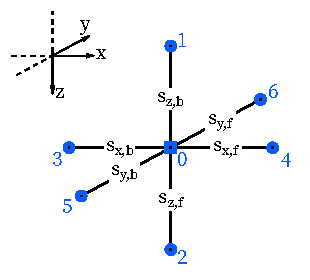
\includegraphics[width=0.7\textwidth]{./0200/grid_stencil_complete.pdf}
        }
    \end{adjustbox}
    \caption[The 7-point stencil used to formulate the central finite differences.]{The 7-point stencil used to formulate the central finite differences for the heat equation around node $0$ (neighbours nodes $1$ to $6$).
    Each $i$-th node corresponds to a value of $T_i$, $k_i$, $A_i$.
    The axis convention is shown in the upper left corner.
    $s_{n,m}$ denotes the grid spacing between nodes, along the $n$-axis and $m$-direction along axis ($b$ backwards, $f$ forwards).}
    \label{suppl:fig:stencil}
\end{figure}

The heat equation under the assumed conditions (Eq.~\ref{suppl:eq:steadystatefullheateq_simplified}) can be formulated using central finite differences for a node and its six neighbours in a 3-D rectangular grid.
The 7-node \textit{stencil} of this nodal configuration (i.e. its graphical representation) is shown in Fig.~\ref{suppl:fig:stencil}.

For any internal node in the model domain

\begin{figure}[hb]
    \begin{adjustbox}{center}
        \fbox{
            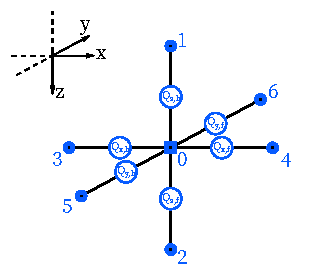
\includegraphics[width=0.7\textwidth]{./0200/grid_stencil_staggered.pdf}
        }
    \end{adjustbox}
    \caption[Additional (staggered) points used in the central finite difference formulation.]{The 6 additional \textit{staggered points} used in the central finite difference formulation, where heat fluxes ($Q_{n,m}$) between node $0$ and its neighbours are expressed.
    The $n$ subscript denotes the axis, the $m$ subscript the along-axis direction ($b$ backwards, $f$ forwards).}
    \label{suppl:fig:stencil_staggered}
\end{figure}

% qui soluzione, anche se lunga (tutta esplicita)
%   ricordare: riferimento in Gerya per heat equation è più avanti
%   se non ricordo male!

% qui passaggio a sistema equazioni lineari

% dopo: boundary conditions

% dopo: assi, indicizzazione

\begin{figure}[hb]
    \begin{adjustbox}{center}
        \fbox{
            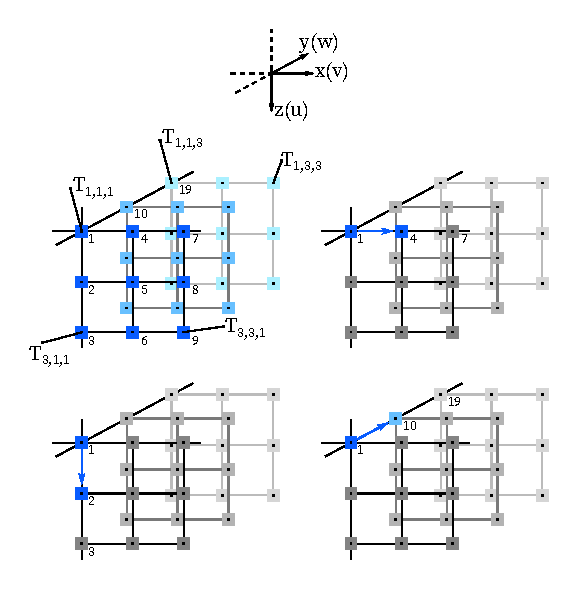
\includegraphics[width=\textwidth]{./0200/grid_indexing.pdf}
        }
    \end{adjustbox}
    \caption[Temp short caption.]{Temp long caption.}
    \label{suppl:fig:GridIndexing}
\end{figure}

% dopo: struttura matrice dei coefficienti

% dopo: non-flat bottom and top boundaries

% TITOLO DA DECIDERE
% INOLTRE, SE DECIDO DI LASCIARE FUORI QUESTA SEZIONE
% QUESTO CAPITOLO VA SENZA SECTIONS
% \section{Definition of lithospheric volumes}
% \label{s:ThermModel:MakeVol}
